\documentclass[10pt,a4paper]{article}
\usepackage[latin1]{inputenc}
\usepackage{amsmath}
\usepackage{amsfonts}
\usepackage{amssymb}
\usepackage{graphicx}
\author{Raul Persa, Lukas Vogel}
\title{Datenbanksysteme - �bung 1}
\begin{document}
\maketitle

\section*{Aufgabe 2}
Using a DBMS as may have the following \textbf{advantages}:
\begin{description}
	\item[Redundancy] DBMS allow for easy data redundancy, which in our case is crucial due to the important nature of the data (votes) 
	
	\item[Atomicity] All Votes need to be atomic. There is no such things as "half" a vote. A DBMS can guarantee that.
	
	\item[Consistency] The overall consistency of the votes can be guaranteed ( i.e. the DB is in a valid state at all time)
	
	\item[Isolation] simultaneous voteshave the same impact as if they were sequential
	
	\item[Durability] A once given remains in the database over the duraton of the election.
\end{description}
While those advantages may seen not very important for a small dataset, they are wildly important for a system handling millions of votes per second. A system that can guarantee basic attributes like those mentioned above takes much strain off of the developer and allows him to focus on other important tasks.

A few \textbf{disadvantages} a DBMS might have are:
\begin{description}
	\item[Security costs] Because of the sensitive nature of the information, additional measures need to be taken to ensure the security of the system
	\item[Hardware and Software Costs] Although it could be argued that paper voting and analysis is more costly
	\item[Possible DB failure]  infrastructure failure could have dramatic impact, it needs to be mitigated though back-ups and physical redundancy
\end{description}

\section*{Aufgabe 3}
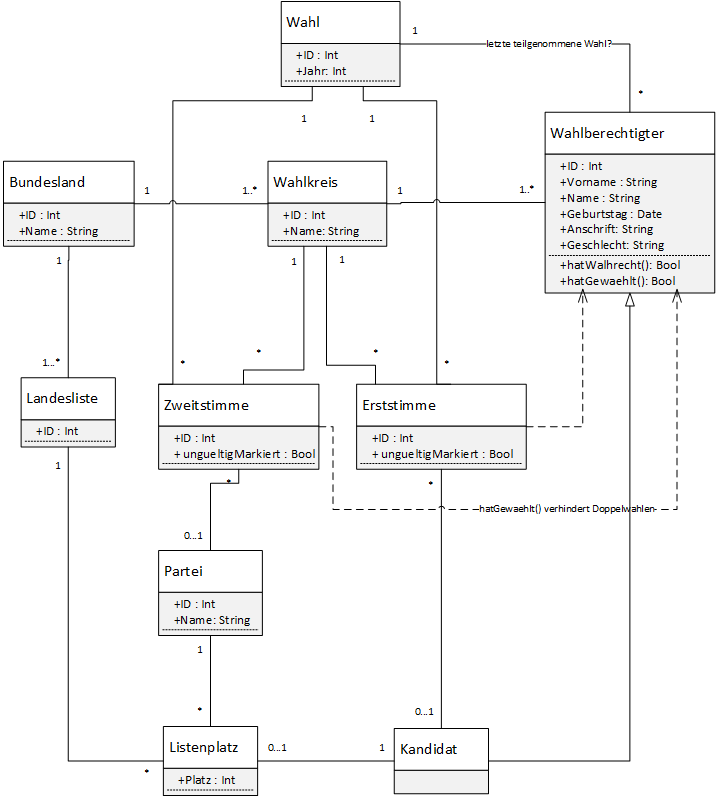
\includegraphics[scale=.8]{../Wahlschema.png}
\end{document}